\documentclass{article}
\usepackage[utf8]{inputenc}
\usepackage{hyperref}

\usepackage{csquotes}
\usepackage{graphicx} % images
\usepackage{subfig} % sub-figures
\usepackage{wrapfig} % wrapping figures
\usepackage[super]{nth} % superscript nth
\usepackage{forest}
\usepackage{pgfgantt}
\usepackage{rotating}
\usepackage{tabularx}
\usepackage{xparse}
\usepackage{booktabs}

\usepackage{adjustbox}
\usepackage{array}
\usepackage{url}

\usepackage{mathptmx}

\usepackage{amsmath,amsfonts,amssymb,amsthm,cancel,icomma,nicefrac,mathrsfs,
            eurosym,verbatim,environ,ifthen,ifdraft,pdfpages,float,booktabs}

\newcommand{\cn}[1]{\textsuperscript{\color{red} ~[citation needed](#1)~}}

\NewDocumentCommand{\rot}{O{90} O{1em} m}{\makebox[#2][l]{\rotatebox{#1}{#3}}}

\title{Master Project Proposal}
\author{Núria Bruch Tàrrega}
\date{January 2020}

\begin{document}

\maketitle
\vspace{20mm}

% !TEX root = ..\main.tex
\section{Project details}
\textbf{Project title}: Measuring the degree of library dependency

\bigskip\noindent
\textbf{Student Name}: Núria Bruch Tàrrega

\href{mailto:nuria.bruch@gmail.com}{nuria.bruch@gmail.com}

\textit{Student id:} 12783145

\bigskip\noindent
\textbf{Host organization}: Software Improvement Group (SIG)

Fred. Roeskestraat 115-123, 1076 EE Amsterdam

\href{https://www.softwareimprovementgroup.com/}{www.softwareimprovementgroup.com}

\bigskip\noindent
\textbf{Contact person}: Lodewijk Bergmans

Senior Researcher

\href{mailto:l.bergmans@sig.eu}{l.bergmans@sig.eu}


\newpage

% !TEX root = ..\main.tex
\section{Project summary} \label{section:project-summary} % Corrector
Nowadays, many open-source libraries are used by developers to be able to reuse the features that these libraries implement.
This implies that a significant number of projects depend on open-source as a concept \cite{kula2014visualizing}.
Maintaining these dependencies and managing the vulnerabilities or problems that these can cause is not a trivial task.

Furthermore, it is a critical task. For example, some vulnerabilities can become security problems that can have a negative impact in terms of integrity, privacy or availability \cite{CVE-FAQ}. This may make it necessary to replace the library being used, to prevent these problems from spreading to the project.

Replacing a library dependency could be a very costly process. For instance, it could involve determining which modules of your project are affected, and which functionalities of the library are being used and need replacement. As well as which is the best way to replace them (i.e. using another library or developing them in-house).
In addition, similar problems may arise if a library becomes closed-source.

Currently, most of the package management systems include dependency management, but these are only listing which dependencies exist in each project \cite{hejderup2018prazi}.
However, a more detailed risk evaluation of the open-source dependencies is missing and could be useful for many projects.
It would be beneficial to analyze the coupling between the project and the libraries that are being used, as well as the effort that replacing a library would involve. It would provide the developers with a more extensive evaluation to be considered when assessing the risk of the project.

This project is carried out in collaboration with the company \textit{Software Improvement Group (SIG)}, and it is motivated by the \textit{FASTEN} project \footnote{\url{https://www.fasten-project.eu/}}. The objective of this project is to improve the quality of open-source development environments to make them more secure and reliable. For this reason, the FASTEN project aims to analyze the software library dependencies that the projects have, in more detail.

\bigskip\noindent
According to the problem described above, we specify the following research questions:

\begin{itemize}
    \item \textbf{RQ1:} How can we measure the degree of source code dependency between a software project and the open-source libraries it uses?
    \item \textbf{RQ2:} How can we measure the effort required to replace the use of an open-source library in a given software project?
\end{itemize}

\newpage
% !TEX root = ..\main.tex
\section{Problem analysis} % Completar i corrector
% Should I add an introduction on how this problem could be interesting to solve to add it to the risk analysis at SIG?

Therefore, as stated with the research questions in section \ref{section:project-summary}, the primary goals of this project are:
Measuring the degree of source code dependency between a project and the libraries it uses, as well as measure the effort needed to replace these libraries.

\subsection{Measuring the degree of source code library dependency}
To the best of our knowledge, there are no papers about measuring the degree of dependency between two separate projects. However, it is true that the degree of dependency between two classes or modules of the same project has already been measured many times, using coupling metrics \cite{yu2011measurement}.

Therefore, we propose re-using the already existing coupling metrics, meant to measure the coupling between units of the \textit{same} project and adapt them to measure coupling \textit{between} projects.

\bigskip\noindent
According to Poshyvanyk and Marcus in \cite{poshyvanyk2006conceptual}, there are five main groups of coupling metrics:

\begin{itemize}
  \item \textbf{Structural coupling metrics:} Measured directly from static source code analysis. Largely studied by the related literature.

  \item \textbf{Dynamic coupling measures:} Measured using dynamic code analysis. "Introduced as the refinement to existing coupling measures due to gaps in addressing polymorphism, dynamic binding, and the presence of unused code by static structural coupling measures" \cite{poshyvanyk2006conceptual}.

  \item \textbf{Evolutionary and Logical coupling:} According to \cite{zimmermann2005mining}, evolutionary coupling can: "tell us which parts of the system are coupled by common changes or cochanges."

  \item \textbf{Coupling measures based on information entropy approach:} Coupling metrics based on the information-theory approach, such as the metrics proposed by Allen and Khoshgoftaar in \cite{allen1999measuring}.

  \item \textbf{Coupling metrics for specific types of software applications:} Specialized coupling metrics for certain types of projects, such as knowledge-based systems or aspect-oriented approach.
\end{itemize}

\bigskip\noindent
The last category is much more domain-specific. Moreover, the evolutionary coupling is not possible to be applied in our context since it is very likely that the separate projects are not going to evolve at the same time, given that they are not developed by the same team. Therefore, the research of this project, owing to the time limitation, is going to be centered on the structural metrics.

These metrics are going to be proposed as a first step to measure the degree of library dependency. These metrics can be extended and calculated more accurately by adding dynamic coupling and information entropy approach metrics if time permits or in future work.

\subsubsection{Structural coupling metrics}
There are many structural coupling metrics, each one measuring a different type of coupling from a different perspective, depending on the purpose for which the metrics are needed.
To decide which metrics can be applied to answer RQ1, we have compared all the metrics according to the papers from Briand et al. \cite{briand1999unified}, Poshyvanyk et al. \cite{poshyvanyk2006conceptual}, and Harrison et al. \cite{harrison1998coupling}. Based on the contents of these papers, we have created Table \ref{table:coupling-metrics}.

The empty cells in Table \ref{table:coupling-metrics} mean that the characteristic is unspecified for the metric in the papers. The \textit{Types of connections} assigned in Table \ref{table:coupling-metrics} as numbers correspond to the descriptions specified in Table \ref{table:types-connections}.

In the same way, the column \textit{Counting connections} has values from A to F, the meaning of which can be found in Table \ref{table:counting-connections}.
The content of both tables, more detailed descriptions, as well as a complete comparison between each type of connection and each way of counting connections, can be found in \cite{briand1999unified}.

\begin{table}[ht!]
    \begin{center}
    \begin{tabularx}{\textwidth}{|l|l|l|X|}
    \hline
    \# & Client Item & Server Item & Description \\
    \hline\hline
    1   & attribute \textit{a} of a class \textit{c} & class \textit{d}, d != c & class \textit{d} is the type of \textit{a} \\
    \hline
    2   & method \textit{m} of a class \textit{c} & class \textit{d}, d != c  & class \textit{d} is the type of a parameter of \textit{m}, or the return type of \textit{m} \\
    \hline
    3   & method \textit{m} of a class \textit{c} & class \textit{d}, d != c  & class \textit{d} is the type of a local variable of \textit{m} \\
    \hline
    4   & method \textit{m} of a class \textit{c} & class \textit{d}, d != c  & class \textit{d} is the type of a parameter of a method invoked by \textit{m} \\
    \hline
    5   & method \textit{m} of a class \textit{c} & \begin{tabular}[c]{@{}l@{}}attribute \textit{a} of a\\ class \textit{d}, d != c \end{tabular}  & \textit{m} references \textit{a} \\
    \hline
    6   & method \textit{m} of a class \textit{c} & \begin{tabular}[c]{@{}l@{}}method \textit{m'} of a\\ class \textit{d}, d != c \end{tabular} & \textit{m} invokes \textit{m'} \\
    \hline
    7   & class \textit{c} & class \textit{d}, d != c  & high-level relationships between classes, such as \textit{uses} or \textit{consists-of} \\
    \hline
    \end{tabularx}
    \end{center}
    \caption{Types of connections, obtained from \cite{briand1999unified}}
    \label{table:types-connections}
\end{table}

\begin{table}[htb!]
    \begin{center}
    \begin{tabularx}{\textwidth}{|l|l|X|}
    \hline
    \begin{tabular}[c]{@{}l@{}}Counting\\ connections\end{tabular} & Level & Description \\
    \hline\hline
    A   & \begin{tabular}[c]{@{}l@{}}Method or\\ attribute\end{tabular} & count individual connections  \\
     \hline
    B   & \begin{tabular}[c]{@{}l@{}}Method or\\ attribute\end{tabular} & count the number of distinct items at the other end of the connections  \\
     \hline
    C   & Class & add up the number of connections counted as in A) for each method or attribute of the class   \\
     \hline
    D   & Class & add up the number of connections counted as in B) for each method or attribute of the class   \\
     \hline
    E   & Class & count the number of distinct items at the end of connections starting from or ending in methods or attributes of the class    \\
     \hline
    F   & Class & for a class c, count the number of other classes to which there is at least  one connection  \\
    \hline
    \end{tabularx}
    \end{center}
    \caption{Counting connections, obtained from \cite{briand1999unified}}
    \label{table:counting-connections}
\end{table}

\begin{table}[p]
    \begin{center}
    \begin{tabular}{|l|l|l|l|l|l|l|}
    \hline
    \rot{Metric} & \rot{Inheritance} & \rot{Import or export} & \rot{Types of connection} & \rot{Domain of measure} & \rot{Counting connections  } & \rot{Indirect coupling} \\ \hline \hline
    CBO & both & both & 5, 6 & class & F & no \\
    CBO' & no & both & 5, 6 & class & F & no \\
    \hline
    $RFC_\alpha$ & both & import & 6 & class & E & depends \\
    RFC & both & import & 6 & class & E & no \\
    RFC' & both & import & 6 & class & E & yes \\
    \hline
    MPC & both & import & 6 & class & C & no \\
    \hline
    DAC & both & import & 1 & class & C & no \\
    DAC' & both & import & 1 & class & D & no \\
    \hline
    COF & no & both & 5, 6 & system & F & no \\
    \hline
    ICP & both & import & 6 & method, class, set & A, C & no \\
    IH-ICP & only & import & 6 & method, class, set & A, C & no \\
    NIH-ICP & no & import & 6 & method, class, set & A, C & no \\
    \hline
    IFCAIC & no & import & 1 & class &  & no \\
    ACAIC & only & import & 1 & class &  & no \\
    OCAIC & no & import & 1 & class &  & no \\
    FCAEC & no & export & 1 & class &  & no \\
    DCAEC & only & export & 1 & class &  & no \\
    OCAEC & no & export & 1 & class &  & no \\
    \hline
    IFCMIC & no & import & 2 & class & C & no \\
    ACMIC & only & import & 2 & class & C & no \\
    OCMIC & no & import & 2, 6 & class & C & no \\
    FCMEC & no & export &  & class & C & no \\
    DCMEC & only & export &  & class & C & no \\
    OCMEC & no & export &  & class & C & no \\
    \hline
    OMMIC & no & import &  & class & C & no \\
    IFMMIC & no & import & 6 & class & C & no \\
    AMMIC & only & import & 6 & class & C & no \\
    OMMEC & no & export & 6 & class & C & no \\
    FMMEC & no & export & 6 & class & C & no \\
    DMMEC & only & export & 6 & class & C & no \\
    \hline
    \end{tabular}
    \end{center}
    \caption{Coupling metrics comparison}
    \label{table:coupling-metrics}
\end{table}

\bigskip\noindent
The first metric of Table \ref{table:coupling-metrics} is CBO which stands for \textit{Coupling between Objects}. This metric counts the number of other classes to which it is coupled, the revised definition of the metric \cite{chidamber1994metrics}, includes inheritance. The revised version of the metric is CBO in Table \ref{table:coupling-metrics}, while the initial definition is CBO'.

The second group of metrics in the table are the \textit{Response for Class} metrics. This metric calculates the response set of a class. According to \cite{chidamber1994metrics}: \textit{"The response set of a class is a set of methods that can potentially be executed in response to a message received by an object of that class"}. The return set includes the methods called directly by the class, as well as the methods that are called by transitivity. In \cite{briand1999unified} it is considered that the inherited methods should be included in this set since they can be executed to respond to a message received in the class. Based on this definition, there are three defined metrics, the first one being $RFC_\alpha$ \cite{churcher1995towards}. The $\alpha$ defines the number of nested levels considered in the calculation of the metric. The other two metrics are particular cases of this one: RFC corresponds to when $\alpha = 1$, and RFC' when $\alpha = \infty$.

The metric \textit{Message Passing Coupling} (MPC) \cite{li1993object} counts invocations from a class to methods of other classes, only from new methods of the class. This means that the inherited methods are not considered. In \cite{briand1999unified}, the definition was modified to \textit{"the number of static invocations of methods not implemented in c by methods implemented in c"}. With the new definition, the ambiguity is eliminated about how to treat overridden methods as well as calls to inherited methods.

Next, there is the group \textit{Data Abstraction Coupling} (DAC) \cite{li1993object}. Because of the uncertainty in the original definition of this metric, in \cite{briand1999unified} the metric is redefined as follows: \textit{"DAC is the number of not inherited attributes that have a class as their type. The number of the classes used as types for attributes is counted by DAC'"}.

The only metric of which the domain of measurement is the entire system is the \textit{Coupling Factor} (COF) \cite{abreu1995toward}. COF calculates the number of relations between classes of the system, which are not related through inheritance. The factor is normalized between 1 and 0 by dividing the number of relations by the maximum number of relations possible in the system. This way, it is possible to compare systems of different sizes.

The following group of metrics contains the metrics for \textit{Information-flow-based Coupling} (ICP). The original ICP metric counts \textit{"for method m of class c, the number of polymorphistically invoked methods of other classes, weighted by the number of parameters of the invoked method."}. From this description, the metric IH-ICP counts only inheritance-based coupling, whereas NIH-ICP counts coupling to those classes with which there is no inheritance relationship. The metric ICP is the sum of the previous two.

The rest of the metrics from Table \ref{table:coupling-metrics} are the suite of metrics defined by Briand et al. \cite{briand1997investigation}.To interpret the metrics suggested by Briand et al. \cite{briand1997investigation}  (from IFCAIC to DMMEC in Table \ref{table:coupling-metrics}), it is necessary to know they are named according to three variables: relationship, locus, and type. The name of each metric is composed in the following way, the initials of the relationship, the initials of the type of interaction, and the initials of the locus. These initials are described below.

\bigskip\noindent
There are three types of relationships, listed below, which can be used to determine the coupling of a class $c$. All the definitions have been obtained from \cite{briand1997investigation}.

\begin{itemize}
  \item Inheritance (A, D): Interactions from a class to its antecessors or descendents, depending on the locus.
  \item Friendship (F, IF): Extension for C++, interactions from class to all the  classes declared as friends or the classes that declare it their friend (inverse friends), depending on the locus.
  \item Other (O): interaction with classes that do not have an inheritance or friendship relationship.
\end{itemize}

\bigskip\noindent
The three different types of interaction descibed by Briand et al. \cite{briand1997investigation}, are the following:
\begin{itemize}
    \item Class-Atribute (CA): "There is a class-attribute (CA-) interaction from class c to class d, if an attribute of class c is of type class d."
    \item Class-Method (CM): "There is a class-method (CM-) interaction from class c to class d, if a newly defined method of class c has a parameter of type class d."
    \item Method-Method (MM): "There is a method-method (MM-) interaction from class c to class d, if a method implemented at class c statically invokes a method of class d (newly defined or overriding), or receives a pointer to such a method."
\end{itemize}

\bigskip\noindent
Finally, the two types of locus are:
\begin{itemize}
  \item Export from a class (EC): "Change flows away from a class", related to the descendants (D) and the friends (F).
  \item Import to a class (IC): "Change flows towards a class", related to the antecesors (A) and the inverse friends (IF).
\end{itemize}

\bigskip\noindent
Now that the metrics have been explained with the tables and the description of each of the metrics, we have to select the candidates to be used in the project.

To begin with, the metric COF is calculating the factor of coupling of a system, only within the given system. However, it is not applicable in our case since we need to calculate the coupling between two systems.
In Table \ref{table:coupling-metrics}, there are some metrics that incorporate inheritance to calculate coupling and some that do not.
Since we want to take into account each usage of the libraries in the projects, it is significant to measure both, inheritance and non-inheritance.
Therefore, the metrics CBO', IH-ICP and NIH-ICP will not be used for this project. The metrics by Briand et al. either only take the inheritance into account or not at all, but they can be combined to consider every type of dependency.

Furthermore, to take the \textit{transitive} dependencies into account, it is important to count transitive coupling as well.
In this manner, the metric $RFC_\alpha$ is truly interesting in this context.
In addition, the metric CBO does not consider multiple connections between the same two classes. Instead, CBO performs a binary evaluation, calculates if a connection exists or not. Therefore, since the goal in this project is to conduct a more fine-grained evaluation of the coupling between the packages, this metric is not applicable.

Finally, the metrics that are being considered for this project, taking into account the criteria explained above, are the following:

\begin{itemize} % Revise definitions to see if it is necessary to discard more measures.
    \item $RFC_\alpha$
    \item MPC
    \item DAC, DAC'
    \item ICP
    \item Metrics by Briand et al. (only for one of the locus)
\end{itemize}

\paragraph{Measuring coupling between software products}
All the metrics described in this section, calculate the coupling at method, class, or set level. However, in the use case of this project, it is necessary to calculate the coupling between two different software products. To do so, we are going to look at how are package-level coupling metrics defined.

Martin in \cite{martin1994oo}, defines two metrics to measure coupling for a group of classes (e.g. packages). Afferent and efferent coupling (Ca and Ce, respectively). Ca is defined as \textit{"The number of classes outside this category that depend upon classes within this category"}, while the description of Ce is \textit{"The number of classes inside this category that depend upon classes outside this category"}. A similar idea is described in \cite{briand1999unified}, there Briand et al. specify that for each coupling there is a client and a server, the dependency has a direction. The problem with the metrics defined by Martin, is that it is not specified what creates a dependency between two classes. That is why, the metrics discussed earlier are interesting for the project in hand, the ambiguity is removed from the description of these metrics, so that they can be understood and calculated.

To use the metrics in a larger domain than the one these are defined to, it is necessary to define an aggregation method. In \cite{briand1999unified}, Briand et al. state \textit{"Of course, measures for smaller domains such as the class level can easily be extended to larger domains like the sets of classes and the system level."}, however, there is no specification of how can this be done.
Nevertheless, in \cn{Lee et al.} it is explained that the coupling of a set of classes, is calculated according to the sum of the coupling of each of the classes. Following this strategy, the calculation of the coupling between two software projects would be the following: First, calculate the coupling of each of the methods of one product with each of the methods of the other product. Then, sum the results of each of the calculations.

Finally, Grupta and Chhabra in \cite{gupta2009package} define the \textit{Package Coupling Metric} (PCM). This metric is defined based on the hierarchical structure of the packages and the dependencies existing on each one of the levels. This strategy of calculating the dependencies of each one of the levels can also be considered when aggregating the coupling of the smaller elements (e.g. methods or classes).

\subsection{Measuring the effort needed to replace a library}
The typical way of estimating effort is by the means of models such as COCOMO II \cite{sharma2011analysis}, which calculate the effort to generate new code. However, for the second research question, it is necessary to find a way to calculate the effort to modify the existing code instead of developing new code. In \cite{kama2014cochcomo} and \cite{asl2013change}, Kama et al. present a tool for software change effort estimation, based on COCOMO II.

This tool, COCHCOMO, combines static and dynamic software analysis to calculate the effort to modify a part of the code. It takes the classes affected by the change into account, both directly and indirectly.

However, COCHCOMO is based on the requirements of the system. Given a change in a requirement, it estimates the effort needed to carry out the change, considering the classes affected by the requirement. The calculation process used in COCHCOMO could be adapted to base it on the replacement a library, instead of basing it on changes in the requirements.

It is also important to consider some new parameters added to this effort calculation. For instance, if the library is deemed to be replaced by another library (or multiple ones) or the features used from the library will be implemented in-house.

Plus, in \cite{kama2014cochcomo} the methodology contemplates the state of each of the classes (i.e. it is finished, in development or not started). It will be examined if this consideration is applicable in the case of this project or not.

\subsection{Proof-of-Concept}
To calculate the metrics as a proof-of-concept, it is necessary to create a dependency graph of the project. It has to be a call-level graph since we require a fine-grained analysis of the source code dependencies. Moreover, it has to represent the software ecosystem of the project considering the various versions of the libraries it uses. This way, it will avoid creating false-positives with library versions the project does not really use.

Most of the literature about modeling software ecosystems, use the nodes of the dependency graph to represent libraries or versions of these \cite{decan2017empirical, hejderup2015dependencies, kikas2017structure}. They are using a package-based approach. The problem with this approach is that, by using this node definition, it is not possible to determine which parts of the project are affected by a particular dependency. The same happens with measuring this dependency. Furthermore, a package-based graph could define transitive dependencies that do not really exist (see Figure \ref{fig:example-call-based} for an example).

\begin{figure}[ht!]
    \centering
    \fbox{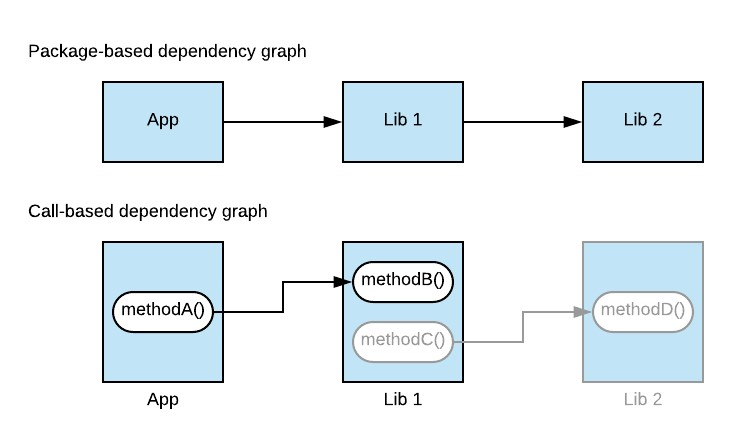
\includegraphics[width=0.8\textwidth]{img/example-call-based.jpg}}
    \caption{Comparison package-based and call-based dependency graphs.}
    \label{fig:example-call-based}
\end{figure}

\bigskip\noindent
Nevertheless, some papers do implement a call-based approach and therefore, could be used in this project.

Hejderup et al. in \cite{hejderup2018software}, propose the creation of a call-level dependency network, in which it can be determined which parts of the project depend on which library. Furthermore, this paper employs a different process to resolve dependencies, taking into account the evolution over time of the versions of the libraries on which the projects depend. Therefore, the analysis of the dependency degree and replacement effort would not be conducted exclusively per library, but also per version of each library.

 Hejderup et al. \cite{hejderup2018prazi}, propose an approach to create a call-based dependency network, PRÄZI. This approach, as the previous one, takes the versioning of the different libraries into account. It also considers that a certain project can depend on various versions of a library at the same time. In the paper, they implement it to create the dependency network of an entire software ecosystem (Crates.io). Nevertheless, this approach could be utilized to construct the network of a given project.

\subsection{Validation of the metrics}
Ultimately, the metrics used in this project will have to be validated. There is not a unique way to validate metrics which is globally accepted and used. Therefore, various approaches will be adopted to validate the metrics as holistically as possible.

In the paper \cite{srinivasan2014software}, Srinivasan et al. explain that there are two fundamental approaches for metric validation: \textit{theoretically} and \textit{empirically}. Therefore, to provide a check of validity that is as broad as possible, a mixture of these two approaches will be used during this project.

For the theoretical validity of the coupling metrics, we will validate that all of them fulfill the \textit{Mathematical Properties of Measures for Coupling}, described in \cite{srinivasan2014software}.

Furthermore, Meneely et al. \cite{meneely2013validating} describe a set of 47 validation criteria for metrics. The time limit of the project does not allow for a complete validation of all the metrics. Consequently, a sub-set of these criteria will be used to validate the metrics. This will be done for both the coupling and effort metrics.

The empirical validation of the metrics will be carried out by the means of case studies. For instance, the predicted effort corresponds to the real required effort, within a certain error window.


% !TEX root = ..\main.tex
\section{Research method} % Started
The main research method that is going to be employed during this project is \textit{Technical Action Research} (TAR) \cite{wieringa2012technical}.

This research method is artifact-based, which means that the first step is to produce the artifact meant to be used in certain situations envisioned by the researcher. The testing of this artifact, to see if it is effective in these situations, is done through a number of iterations. First, under ideal conditions, and then changing the experiments step by step to reach a real-world situation. These iterations, in the context of this project, are going to be limited due to the existing deadlines. However, there is the option of continuing with this part of the work in the future.

\bigskip\noindent
In addition, the research will also include controlled experiments. These experiments will be conducted as the empirical part of the validation of the coupling metrics. Additionally, the empirical validation of the effort estimation is going to be achieved by the means of case studies. In these case studies, the estimated effort will be compared with the real effort that the change required.

\bigskip\noindent
Some of the most difficult parts of this research are the validation and adaptation of the coupling metrics.

First, the validation since there is not a unique way to do it, but rather a wide variety of criteria and approaches. Therefore, conducting a complete validation is a complex task as it is not possible to validate every aspect of the metric.

In addition, even though the metrics that are going to be used to measure coupling between the projects and the libraries already exist, they are going to be adapted. These changes of the metrics could be complex for some of them. However, there are many metrics that could be used, and the ones that can not be adapted could serve as an indication of the types of dependencies that could exist when adapting other metrics.

\bigskip\noindent
After the formal definition and theoretical validation of the metrics for both, the coupling measurement and the estimation effort, to replace a library, a Proof-of-Concept (PoC) will be made. With this PoC, the metrics will be calculated for the projects given to the PoC. Once the PoC is ready, the empirical validation will be carried out for each of the metrics, by conducting controlled experiments and case studies as elaborated above.

\bigskip\noindent
The methodology for validating the metrics chosen during this research will be divided into two phases: a first phase of theoretical validation and a second one of empirical validation \cite{srinivasan2014software}.
These validations will be carried out during the phases \textit{Creation of the theoretical model} and \textit{Evaluation of the project} respectively (see Section \ref{section:timeline}).

\paragraph{Literature survey}
During the literature survey for this proposal we mainly utilized \textit{Google Scholar}. The resources found were documented with the following structure: First, by the overarching area of research, in this case: Dependency management, dependency/coupling metrics, effort estimation, and metrics validation.

As for the metrics validation category, we have conducted a brief excerpt of the main points or useful information extracted from each of the papers.
Finally, the papers of coupling metrics are used to extract the characteristics of each of the proposed metrics to filter out the non-applicable metrics (see Table \ref{table:coupling-metrics}). Besides, the effort estimation papers were used as a survey of the major models in order to compare them.

See section \ref{section:literature} for more detail.

\bigskip\noindent
Once the literature survey is finalized, we expect the following input:

\begin{itemize}
  \item A clear overview of the existing coupling metrics, as well as a comparison between them, in order to have the necessary knowledge to determine if a metric is applicable to the situation considered in this project, and how could it be adapted.

  \item The different existing models to estimate effort. An overview of the necessary steps and the data to estimate effort and the differences between the models.

  \item The various approaches to validate metrics, and the different characteristics of the methodologies. Also, the awareness of which methodologies and criteria could be applied to the proposed metrics.

  \item The existing options to create a call-level dependency graph for the PoC.
\end{itemize}

\paragraph{Timeline}
The timeline of this project will be divided in five main parts. A description of each one of these parts can be found in Section \ref{section:timeline}, as well as a timeline in the form of a Gantt diagram, in Figure \ref{figure:gantt-chart}.


% !TEX root = ..\main.tex
\section{Expected results of the project} \label{section:expectedResults}
Currently, there are three expected results of this project:

\paragraph{Theoretical description of the set of metrics:}
The first result is the description of a set of metrics to be used to answer the research questions. These are the coupling metrics to calculate the degree of dependency between a project and its libraries, as well as the estimation of effort needed to replace the libraries.
Each metric will include a formal definition as well as a set of validation criteria that these metrics will have to fulfill to be considered valid.

\paragraph{Implementation of the proof-of-concept (PoC):}
The second result will be the software implementation of the previously created theoretical model.
This PoC will be meant to be used as a prototype to calculate the metrics proposed, to use the results for the evaluation and validation of the metrics.

\paragraph{Validation of the metrics:}
Once the PoC is ready, the validation of the metrics will be conducted. There will be experiments for the coupling metrics, as well as case studies for the effort estimation.
The third result is expected to be a report with the conclusions of the validation, the theoretical and the empirical ones.


% !TEX root = ..\main.tex
\section{Required expertise}\label{section:requiredExpertise}
In this section, the required expertise to carry out this project is discussed.
In Table \ref{table:skills-proficiency}, the necessary skills are listed. Each skill is associated with a \textit{Required proficiency}, which represents the level of knowledge required for the project and the \textit{Current proficiency}. These levels of knowledge are assigned according to the following proficiency scale:

\begin{enumerate}
	\item   Fundamental
	\item   Basic
	\item   Intermediate
	\item   Advanced
	\item   Expert
\end{enumerate}

\begin{table}[ht!]
    \begin{center}
    \begin{tabularx}{\textwidth}{|X|c|c|}
    \hline
    Skill & Required proficiency & Current proficiency \\
    \hline\hline
    Java programming                            & Expert    & Intermediate \\
    \hline
    Static code analysis                        & Advanced  & Basic \\
    \hline
    Software metrics consideration and design   & Intermediate - Advanced  & Basic \\
    \hline
    Software metrics validation                 & Intermediate - Advanced & Basic \\
    \hline
    Open-source implications                    & Intermediate  & Intermediate \\
    \hline
    Software architecture design                & Advanced  & Intermediate \\
    \hline
    %R                                   & Advanced & Basic \\ \hline
  \end{tabularx}
    \end{center}
    \caption{Necessary skills with required and current proficiency}
    \label{table:skills-proficiency}
\end{table}


% !TEX root = ..\main.tex
\section{Timeline}\label{section:timeline}
This project will be divided into several phases:

\begin{enumerate}
    \item \textbf{Learning:} This initial phase consists of acquiring the necessary knowledge to obtain the level of competence required to carry out the project
    (see section \ref{section:requiredExpertise}).

    \item \textbf{Creation of the theoretical model:} In this phase, we will define the metrics to be used to calculate the coupling of a project with the libraries it uses. Also, the model to estimate the effort to replace a library will be defined.

    In addition, the validation criteria that are going to be used for each of the metrics will be described, and the theoretical validation of these metrics will be carried out.

    \item \textbf{Development of the Proof-of-Concept (PoC):} This third phase consists of implementing the PoC to calculate the coupling metrics and to implement the effort estimation model.

    \item \textbf{Evaluation of the project:} In this phase, the PoC will be used in real projects. The results obtained for each one of the metrics, as well as the model of effort estimation, will serve as the data to conduct the empirical validation. This validation will be done by means of controlled experiments and case studies.

    \item \textbf{Thesis writing:} This phase consists of writing down the process of each of the previous phases for the creation of the documentation of the project.
\end{enumerate}

\noindent
It should be noted that the last phase: \textit{Thesis writing}, will not be carried out in a sequential manner with the other phases, but will be done in parallel with the rest of the phases.

During phases 2, 3, and 4, the three expected results of the project will be developed (see section \ref{section:expectedResults}).


\begin{figure}[p]
    \begin{center}
        \rotatebox{90}{\begin{ganttchart}[y unit title=0.4cm,
        y unit chart=0.5cm,
        vgrid,hgrid,
        title label anchor/.style={below=-1.6ex},
        title left shift=.05,
        title right shift=-.05,
        title height=.75,
        bar/.style={fill=gray!55},
        incomplete/.style={fill=white},
        progress label text={},
        group right shift=0,
        group top shift=.25,
        group height=.25]{14}{33}
        %labels
        \gantttitle{Weeks}{19} \\
        \gantttitlelist{14,...,33}{1} \ganttnewline
        %tasks
        \ganttgroup{Learning}{14}{18} \\
            \ganttbar{Static / Dynamic code analysis}{14}{14} \\
            \ganttbar{Software metrics consideration}{15}{15} \\
            \ganttbar{Software Architecture design}{16}{16} \\
            \ganttbar{Library dependency evaluation}{17}{17} \\
            \ganttbar{R coding}{18}{18} \\
        \ganttgroup{Creation of the theoretical model}{19}{22} \\
            \ganttbar{Metrics to calculate the degree of dependence}{19}{20} \\
            \ganttbar{Metrics to calculate change effort}{21}{22} \\
        \ganttgroup{Implementation of the PoC}{23}{27} \\
            \ganttbar{Implementation of the dependency call-graph}{23}{25} \\
            \ganttbar{Implementation of the calculation of the metrics}{25}{26} \\
            \ganttbar{Implementation of the visual representation}{27}{27} \\
        \ganttgroup{Evaluation of the project}{28}{33} \\
            \ganttbar{Validation of code change effort}{28}{31} \\
            \ganttbar{Validation of dependency degree}{32}{33} \\
        \ganttgroup{Thesis writing}{14}{33} \\
            \ganttbar{\textit{Background} Chapter}{14}{18} \\
            \ganttbar{\textit{Set of metrics} Chapter}{19}{22} \\
            \ganttbar{\textit{PoC} Chapter}{23}{28} \\
            \ganttbar{\textit{Evaluation} and \textit{Conclusions} Chapter}{29}{33} \\

        %relations
        %\ganttlink{elem0}{elem4}

        \end{ganttchart}}
    \end{center}
    \caption{Gantt Chart}
    \label{figure:gantt-chart}
\end{figure}


% !TEX root = ..\main.tex
\section{Risks} % Acabar i corrector
\paragraph{Project goals are too ambitious.}
If the project goals are underestimated, it could cause a problem in terms of project completion.
To minimize the possibility of this risk becoming reality, it is critical to clearly specify the goals of the project.
To be able to react if the risk is not prevented, some extra time has been not included in the planned timeline.
First, more hours could be invested as overtime and weeks 34 and 35 can also be added to the project, while the final deadline would still not be missed.

\paragraph{Project goals are too vague.}
This risk is also related to the definition of the project objectives. As with the previous risk, to prevent it, it is important to dedicate the necessary time and effort to specify the objectives.
However, if this situation is detected, the development of the project will be stopped to reassess and specify the objectives in more detail.
In this way, it will be avoided that this risk leads to major problems in later stages of the project.

\paragraph{The information about the project is unavailable/incomplete/too difficult.}
In order for this risk not to lead to severe problems during the project, it is important to gather information on the topic as soon as possible.
If it is noticed that there is not enough information or the project is overly complex, efforts will be focused on the part of the project that is most feasible.
In this way, the project would be continued; although the result would not be as complete as planned, it would serve as a starting point for future continuation.

\paragraph{The gap between the current expertise and the required expertise is too large.}
To mitigate the possibility that this risk becomes reality and results in a grave problem for the holistic completion of the project,
during the first phase of the project, time has been allocated for knowledge gathering. This is meant to reduce the gap between the required and current knowledge.
In the same way, it could be detected that it is necessary to invest more hours in the training phase.
These hours would be spent in the form of overtime, which would not affect the estimated date of completion of the project.

\paragraph{Adaptation and justification of the coupling metrics.}
During the second phase of the project, the coupling metrics are going to be adapted. One of the risks associated with this task is that the metrics may not be flexible enough to be used in a different context.
To prevent this, we selected several metrics that could be used. Therefore, if one of them is not feasible to adapt, we can use the rest. However, if this is the case, the characteristics of the discarded metric and the type of coupling that it measures would be considered when adapting another metric.

\paragraph{Adaptation of the effort to change code calculation.}
This risk is similar to the previous risk. In this case, we would have to consider an alternative model to estimate the effort to implement in the context studied in this project. To do so, it is important to consult the support from experts in the field of research, as well as the first phase of the project. In this initial phase, it is expected for us to acquire the necessary knowledge about the model to be able to assess if the adaptation is feasible.

\paragraph{Validation of the metrics.}
Since there is no unique and standardized way to validate metrics, this task entails a risk for the project. The validation will be performed for certain properties and validation criteria for each of the used metrics. However, the time limit does not allow for all of the metrics to be validated using each of the criteria, or conduct too many experiments. Therefore, once the project is finalized, we could affirm that the metrics have been validated, but it will not be a complete validation.


% !TEX root = ..\main.tex
\section{Literature survey}\label{section:literature} % Acabar
For the creation of this proposal, we have conducted research on various topics, listed below. For each of these research activities, the tool that has been mainly used is \textit{Google Scholar}.

\begin{itemize}
    \item Dependency management
    \item Coupling metrics
    \item Code change effort measurement
    \item Research methods
\end{itemize}

\noindent
The papers to be used for this document were selected according to their language (English) and accessibility. Of all the performed searches, we first conducted a selection according to titles and a second filter after reading the abstract and introduction of the papers.

The papers that according to these filters are related and relevant to the topic of this research were completely read and used to create this proposal. For each of the selected papers, the references of the paper were reviewed following the same procedure.

\paragraph{Dependency management}
This topic has been researched from various facets, one of the most widespread being the vulnerability of libraries.
Examples of research on vulnerabilities in libraries and how these are expanded through the projects that utilize them, are \cite{decan2018impact,  hejderup2015dependencies, pashchenko2018vulnerable, plate2015impact}.

Another aspect of the dependencies between projects that have also been studied are the dynamics of usage between packages and versions of these.
For example, Wittern et al. in \cite{wittern2016look} analyze the dynamics of package use in \textit{npm} and the adoption of new versions of these by the developers.
Plus, Mileva et al. analyzed the popularity of library versions, as well as the adoption process of them \cite{mileva2009mining}.

Ultimately, there is research related to modeling software ecosystems, such as \cite{decan2017empirical, hejderup2015dependencies, kikas2017structure}. However, most of these models are created at a project or project version level.

\bigskip\noindent
There are no studies, that we have been capable to find, analyzing the degree of dependence of a project on the libraries that it uses. This fact was perceived by Hejderup et al in \cite{hejderup2018software}.

\paragraph{Coupling metrics}
To obtain the papers describing the coupling metrics to be used in this project, we initially found the papers about measuring dependency (e.g. \cite{cataldo2009software, poshyvanyk2006conceptual}). Based on these papers, the research was focused on structural coupling metrics, which lead to finding the literature review papers and the definition of the metrics (e.g. \cite{briand1997investigation, briand1999unified, harrison1998coupling}).

Finally, we conducted a literature survey focused on how to validate the metrics. Resulting in papers about the diverse approaches and properties of the metrics to take into account when conducting a validation. For instance, \cite{meneely2013validating, roche1994software, srinivasan2014software}.

\paragraph{Code change effort measurement}
To gather information about the techniques to estimate effort, the first step was to research about the general topic effort estimation, yielding papers such as \cite{sharma2011analysis}.
Next, the research focused on estimating effort to change code, providing as principal result the research by Kama et al. in \cite{kama2013integrated, kama2014cochcomo}.

\paragraph{Dependency graphs}
To create the PoC, it is necessary to implement a dependency graph that permits the calculation of the metrics. The first results obtained during the literature survey about dependency graphs (e.g. \cite{kikas2017structure, kula2017modeling}) used package-based approaches. Therefore, we limited the search to call-based approaches. The two main results of this final search have been \cite{hejderup2018prazi, hejderup2018software}.

\paragraph{Research methods}
In this case, the first paper used to define the research method of the project, was given by the university. In \cite{easterbrook2008selecting} a description of each of the main research methods can be found. Based on this paper, the research was focused on papers about the research methods selected to be used during this project (e.g. \cite{wieringa2012technical}).


\newpage

\bibliographystyle{plain}
\bibliography{references}

\end{document}
